\documentclass[a4paper, 12pt]{article}
\usepackage{a4wide}
% Необходимые пакеты для компиляции русского языка, картинок и прочего

\usepackage[utf8]{inputenc}                % Кодировка
\usepackage[main=russian, english]{babel}  % Русский язык
\usepackage[pdftex]{graphicx}              % Картинки
\usepackage{indentfirst}                   % Отступ перед абзацами

\usepackage{amsmath}  % Математические 
\usepackage{amssymb}  % формулы

\usepackage{tikz}                % Векторная графика
                                 %
\usepackage{pgfplots}            % % Нужно для вставки графиков из 
\pgfplotsset{compat=newest}      % % matlab2tikz
\usepgfplotslibrary{groupplots}
\usepgfplotslibrary{dateplot}
\usetikzlibrary{plotmarks}       % %
\usetikzlibrary{arrows.meta}     % %
\usepgfplotslibrary{patchplots}  % %
\usepackage{grffile}             % %

\usepackage{caption} % Чтобы можно было вставлять формулы к подписям рисунков

\usepackage[unicode]{hyperref}                                         % Ссылки и русские закладки
\hypersetup {                                                          %
    pdftitle={Отчёт по практикуму},                                    % Название документа
    pdfsubject={Динамическое программирование и процессы управления},  % Тема документа
    pdfauthor={Егоров Кирилл Юлианович},                 % Автор документа
    pdfcreator={Кафедра системного анализа ВМК МГУ},     % Создатель документа
    pdfproducer={LaTeX},                                 % Программа, создавшая документ
    hidelinks                                            % Скрывает рамку вокруг ссылок
}


\usepackage{nicefrac}
\usepackage{amsthm}  % Красивый внешний вид теорем, определений и доказательств
\newtheoremstyle{def}
        {\topsep}
        {\topsep}
        {\normalfont}
        {\parindent}
        {\bfseries}
        {.}
        {.5em}
        {}
\theoremstyle{def}
\newtheorem{definition}{Определение}
\newtheorem{example}{Пример}

\newtheoremstyle{th}
        {\topsep}
        {\topsep}
        {\itshape}
        {\parindent}
        {\bfseries}
        {.}
        {.5em}
        {}
\theoremstyle{th}
\newtheorem{theorem}{Теорема}
\newtheorem{lemma}{Лемма}
\newtheorem{assertion}{Утверждение}

\newtheoremstyle{rem}
        {0.5\topsep}
        {0.5\topsep}
        {\normalfont}
        {\parindent}
        {\itshape}
        {.}
        {.5em}
        {}
\theoremstyle{rem}
\newtheorem{remark}{Замечание}

% Новое доказательство
\renewenvironment{proof}{\parД о к а з а т е л ь с т в о.}{\hfill$\blacksquare$}

\begin{document}
    \thispagestyle{empty}
\begin{center}
    \ \vspace{-3cm}

    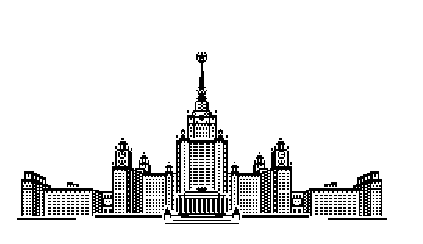
\includegraphics[width=0.5\textwidth]{title_page/msu.eps}\\

    {\small{\scshape  Московский государственный университет имени М. В. Ломоносова}\\
    Факультет вычислительной математики и кибернетики\\
    Кафедра системного анализа}

    \vfill

    {\Large Практикум}

    \vspace{1cm}

    {\LARGE\bfseries <<Элементы финансовой математики>>}

    \vspace{1.5cm}

\end{center}

\vspace{3cm}

\begin{flushright}
    \large
    \textit{Студент 515 группы}\\
    К. Ю. Егоров

    \vspace{5mm}
    
    \textit{Руководитель практикума}\\
   к.ф.-м.н., доцент С. Н. Смирнов
\end{flushright}

\vfill

\begin{center}
    Москва, 2022
\end{center}

\clearpage
    \tableofcontents
    \newpage

    \section{Постановка задачи}
    Рассматривается задача суперхеджирования опциона Call~On~Max американского типа с ценой исполнения $\chi > 0$ и функцией выплат
    \begin{equation}\label{eq:call_on_max}
        \begin{cases}
        g_t(\bar x_t) = \mathrm{max}\{\mathrm{max}\{x^1_t,x^2_t,\ldots,x^n_t\} - \chi,\,0\},\;\mbox{при $t=1,2,\ldots,T,$}\\
        g_0(\bar x_0) = -\infty,
        \end{cases}
    \end{equation}
    для $n = 2$ рисковых активов при наличии торговых ограничений. Время~$t$ в задаче принимается дискретным, неотрицательным и ограниченным горизонтом~$T$.

    Положительный вектор $x_t=(x^1_t,x^2_t,\ldots,x^n_t) > 0$ обозначает дисконтированные цены рисковых активов в момент времени~$t$. За $\bar x_{t-1} = (x_0,x_1,\ldots,x_{t-1})$ обозначим предысторию цен, сложившуюся к моменту времени~$t$. Также считаем, что цена безрискового актива постоянна, равна единице, а торговые ограничения для него отсутствуют.

    Стратегией хеджера называется последовательность векторов $h_1,h_2, \ldots, h_T$, удовлетворяющая торговым ограничениям, заданным многозначным отображением $D_t(\cdot)$:
    \begin{equation}
        h_t \in D_t(\bar x_{t-1}) \subseteq \mathbb{R}^n.
    \end{equation}

    Динамика цен описывается мультипликативной моделью:
    \begin{equation}
        x_t = m_t \odot x_{t-1},\;\mbox{где $m_t \in E_t(\bar x_{t-1})$.}
    \end{equation}
    Здесь $\odot$ обозначает поэлементное произведение векторов, а $E_t(\cdot)$~--- компактнозначное отображение, задающее ограничения на мультипликаторы. По условию задачи, $E_t(\cdot) \equiv \Pi$, где $\Pi = [a,b]\times[c,d]$~--- прямоугольник, $0<a<b$, $0<c<d$. Параметры множества~$\Pi$ выбираются таким образом, чтобы $\Pi \subset \mathbb{R}^n_+$ и выполнялось условие отсутствия гарантированного арбитража с неограниченной прибылью \textit{NDSAUP}, то есть когда
    \begin{equation}\label{eq:no_arbitrage}
        \mathrm{conv}K_t(\cdot) \cap \mathrm{bar}D_t(\cdot) \neq \varnothing,\;\mbox{где $K_t(\bar x_{t-1}) = (\Pi - \bar 1) \odot x_{t-1}$}.
    \end{equation}
    Здесь отображение~$K_t(\cdot)$ задает ограничения для данной модели, если записать её в аддитивной форме:
    \begin{equation}
        x_t = x_{t-1} + y_t,\;\mbox{где $y_t \in K_t(\bar x_{t-1})$.}
    \end{equation}

    Целевая функция~$v^*_t(\bar x_t)$~--- это резервы, необходимые для покрытия обязательств по проданному опциону. Целевая функция~$v^*_t(\bar x_t)$ удовлетворяет уравнению Беллмана--Айзекса (мы считаем, что выполнены необходимые условия полунепрерывности сверху функции $v^*_t(\bar x_t)$):
    \begin{equation} \label{eq:bellman-ajzeks}
        \begin{cases}
            v^*_t(\bar x_t) = g_{t-1}(\bar x_{t-1}) \lor \mathrm{sup}_{Q \in \mathcal{P}_t^n(\bar x_{t-1})} \left\{
                \int v_t^*(\bar x_{t-1},\, x_{t-1}+y)\,Q(dy)
                -
                \rho\left(
                    \left. \int y\,Q(dy)
                    \right|
                    D_t(\bar x_{t-1})
                \right)
            \right\}, \\
            v_T^*(\bar x_T) = g_T(\bar x_T),
        \end{cases}
    \end{equation}
    где $\rho\left(\cdot\left| D_t(\bar x_{t-1}) \right.\right)$ обозначает опорную функцию множества~$D_t(\bar x_{t-1})$, а $\mathcal{P}_t^n(\bar x_{t-1})$~--- все вероятностные меры, носители которых вложены в~$K_t(\bar x_{t-1})$ и состоят не более, чем из $(n+1)$ точки. Отметим также, что данный подход позволяет разделить задачи ценообразования и хеджирования.

    Целью данной практической работы является нахождение решения уравнения Белл\-мана--Айзекса и анализ качественного поведения премии за опцион $v_0^*(x_0)$ в зависимости от следующих факторов:
    \begin{enumerate}
        \item начальных цен рисковых активов,
        \item дисперсии цен активов,
    \end{enumerate}
    при вариантах торговых ограничений $D_t(\cdot)$:
    \begin{enumerate}
        \item отсутствие торговых ограничений,
        \item запрет коротких позиций по обоим активам,
        \item запрет коротких позиций по более волатильному активу,
        \item запрет коротких позиций по менее волатильному активу.
    \end{enumerate}


    \section{Условие безарбитражности}
    Заметим, что условие безарбитражности~\eqref{eq:no_arbitrage} будет выполнено для любых торговых ограничений $D_t(\cdot)$, если оно выполнено для случая без торговых ограничений~$D_t(\cdot) \equiv \mathbb{R}^n$. Тогда $\mathrm{bar}\mathbb{R}^n = \{0\}$ и получаем
    \begin{equation}
        0 \in (\Pi - \bar 1) \odot x_{t-1},
    \end{equation}
    или, в силу положительности цен,
    \begin{equation}
        \bar 1 \in \Pi.
    \end{equation}

    Таким образом, условие безарбитражности~\textit{NDSAUP} выполнено для любого прямоугольника~$\Pi$ с ограничениями
    $$
        a \leqslant 1,\; b \geqslant 1,
    $$
    $$
        c \leqslant 1,\; d \geqslant 1.
    $$

    
    \section{Алгоритм решения уравнения Беллана--Айзекса}

    Уравнение Беллмана--Айзекса~\eqref{eq:bellman-ajzeks} может быть решено при каждом $t$ в два этапа:
    \begin{enumerate}
        \item для фиксированного $z \in K_t(\bar x_{t-1})$ вычисляется функция
        \begin{equation}
            u_t(\bar x_{t-1}, z) = \mathrm{sup}_{Q\in\mathcal{P}_t^n(\bar x_{t-1}),\, \int yQ(dy)=z}\int v_t^*(\bar x_{t-1}, x_{t-1} + y)\,Q(dy);
        \end{equation}
        \item функция цены находится как
        \begin{equation}
            v_{t-1}^*(\bar x_{t-1}) = g_{t-1}(\bar x_{t-1}) \lor \mathrm{sup}_{z \in K_t(\bar x_{t-1})} \{u_t(\bar x_{t-1}, z) - \rho(z|D_t(\bar x_{t-1})) \}.
        \end{equation}
    \end{enumerate}

    Заметим, что функция $u_t(\bar x_{t-1}, z)$ совпадает в точке~$z$ с вогнутой оболочкой функции
    \begin{equation}
        f(y) = 
        \begin{cases}
            v_t^*(\bar x_{t-1}, x_{t-1} + y),&\mbox{где $y \in K_t(\bar x_{t-1})$};\\
            -\infty, & \mbox{иначе}.
        \end{cases}
    \end{equation}
    При этом в пункте 2 достаточно рассматривать только векторы $z$ из $K_t(\bar x_{t-1}) \cap D_t(\bar x_{t-1})$.

    При построение вогнутой оболочки компакты $K_t(\cdot)$ аппроксимируются (по метрике Хаусдорфа) конечными множествами на сетке $\hat K_t(\cdot)$. Для численного решения использовался комплекс программ «Робастное управление портфелем финансовых инструментов» (версия 0.1.0)\footnote{https://github.com/doctormee/robust-fpm-cmc-msu-edu-2021}. Для перехода от мультипликативной модели с независящими от цен ограничениями к аддитивной модели используется класс MDAFDynamics.

    
    \section{Влияние торговых ограничений}

    Докажем лемму, применив которую, мы сможем существенно сократить количество вычислений.

    \begin{lemma}
        Пусть функция выплат~$g_t(\bar x_t)$ одинакова при всех $t$, зависит только от $x_t$ и неубывает, то есть для любого $y\in\mathbb{R}^n_{+}$ выполнено $g(x_t + y) \geqslant g(x_t)$.
        Тогда премии за опцион совпадают для всевозможных торговых ограничений $D_t(\cdot)$ таких, что $D_t(x_{t-1}) \subseteq \mathbb{R}^n_{+}$.
    \end{lemma}

    \begin{proof}
        С помощью уравнения Беллмана–Айзекса~\eqref{eq:bellman-ajzeks} легко показать по индукции, что функция $v_t^*(\bar x_{t-1}, \cdot)$ также является неубывающей. Её вогнутая оболочка $u_t(\bar x_{t-1}, z)$ также является неубывающей. В силу наложенных на $D_t(\cdot)$ ограничений,
        \begin{equation}
            \mathrm{bar}\,D_t(\bar x_{t-1}) \subseteq \mathbb{R}^n_{-} = \{x \in \mathbb{R}^n\;:\;x_i \leqslant 0,\; i=\overline{1,n}.\}
        \end{equation}
        Таким образом, максимум в (13) достигается на $z = 0 \in K_t(\bar x_{t-1}) \cap \mathrm{bar}\,D_t(\bar x_{t-1})$. В частности, минимум достигается в $z = 0$ в случае отсутствия торговых ограничений, когда $\mathrm{bar}\,D_t(\cdot) = \{0\}$, поэтому значения всех функций $v_t^*$ будут совпадать.

    \end{proof}

    Утверждение леммы можно интерпретировать следующим образом: при суперхеджирования опциона с неубывающей функций выплат хеджер всегда может занимать неотрицательные позиции по всем активам.
    Заданная функция выплат~\eqref{eq:call_on_max} не убывает, поэтому, согласно предыдущей лемме, мы можем строить графики для одного любого из предложенных типов ограничений, остальные обязаны совпасть.
    Далее, если не оговорено обратное, программа работала в режиме без торговых ограничений.
    
    
    \section{Результаты вычислений}
    Ниже представлены результаты работы программы: интересные графики с кратким пояснением происходящего.
    Временной горизонт~$T$ у всех графиков равен $5$.

    \begin{figure}[h]
        \noindent
        \centering
        {
                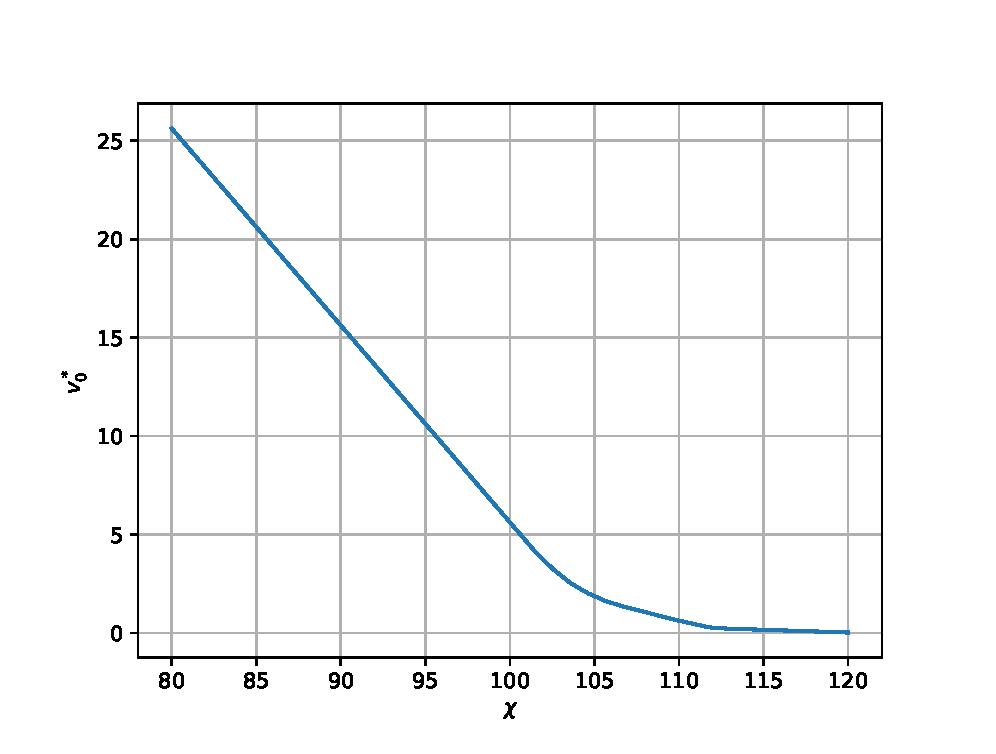
\includegraphics[width=120mm]{depends_on_strike.eps}
        }
        \caption{Зависимость премии за опцион от величины страйка для начальной стоимости $x_0=[100,100]$ и ограничений $\Pi=[0,\!97,1,\!03]\times[0,\!99,1,\!01]$.}
    \end{figure}

    \begin{figure}[t]
        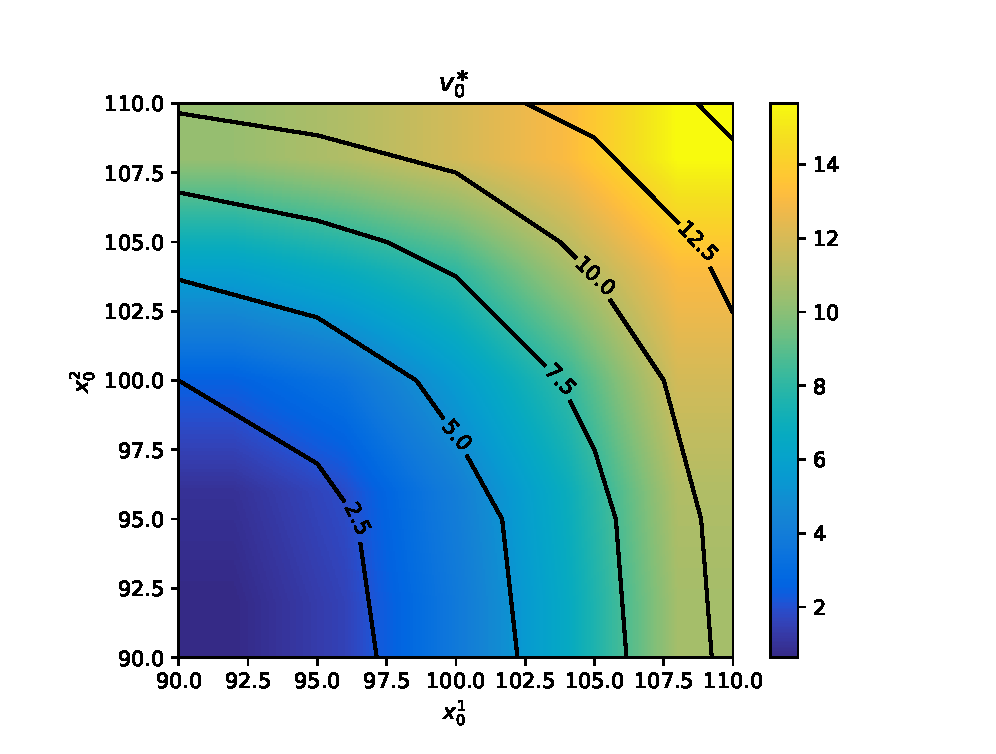
\includegraphics[width=0.5\linewidth]{constraint_no.eps}
        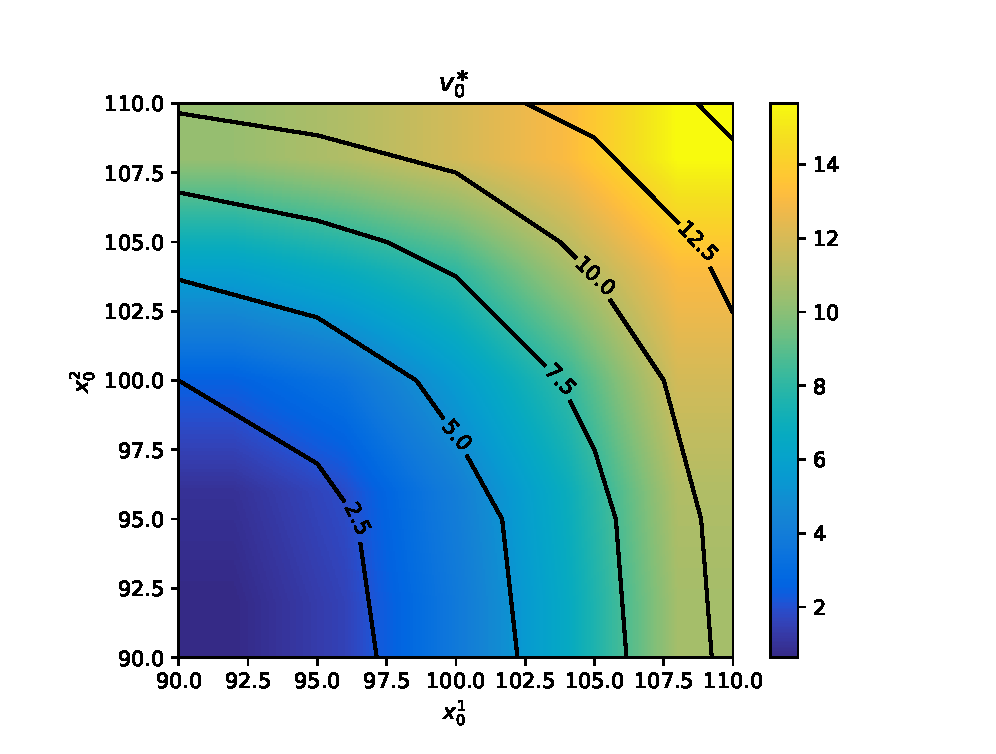
\includegraphics[width=0.5\linewidth]{constraint_all.eps}
        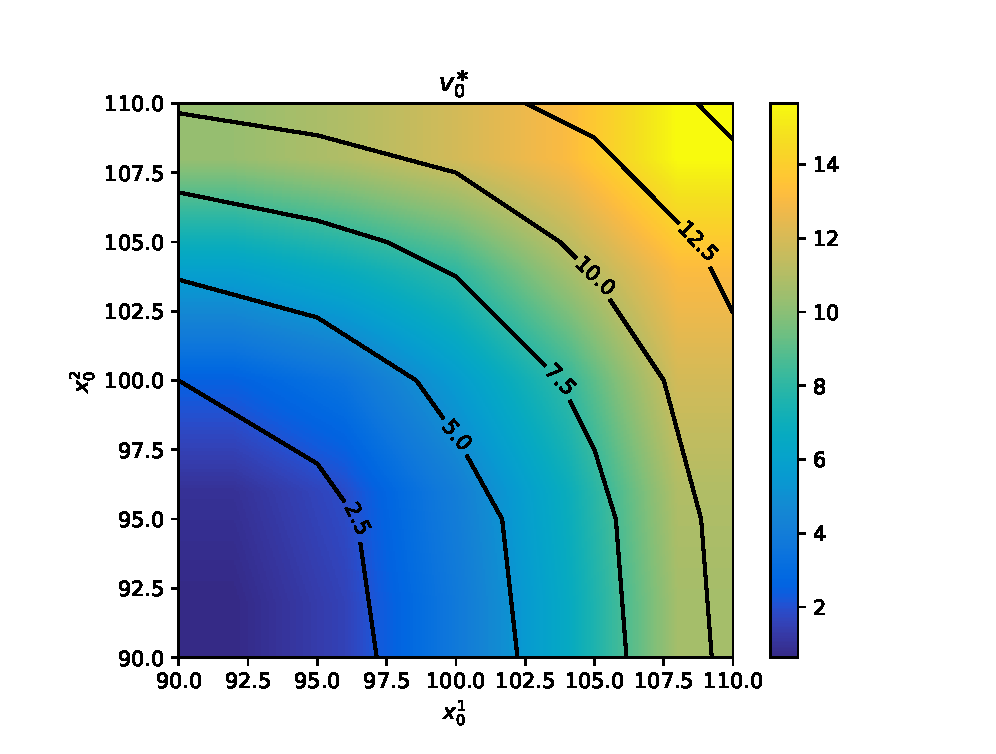
\includegraphics[width=0.5\linewidth]{constraint_more.eps}
        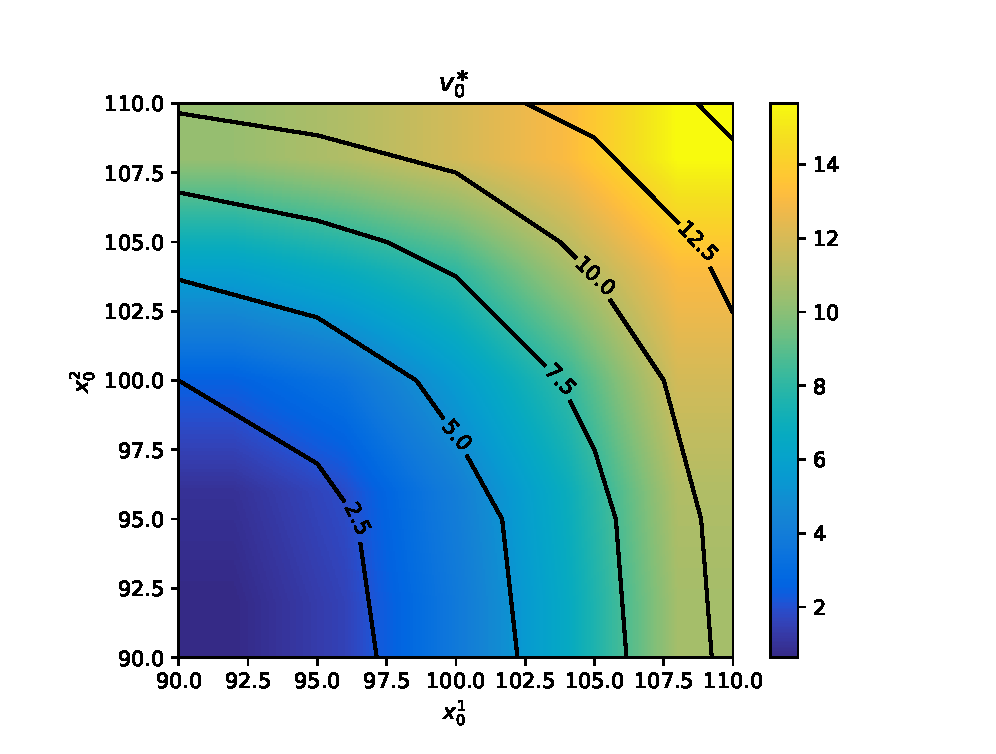
\includegraphics[width=0.5\linewidth]{constraint_less.eps}
        \caption{Зависимость премии от начальной цены активов на крупной сетке для различных типов торговых ограничений: без ограничений, без коротких позиций, без коротких позиций по более волатильному активу, без коротких позиций по менее волатильному активу. Здесь ограничения задаются как $\Pi=[0,\!97,1,\!03]\times[0,\!99,1,\!01]$. Видно что графики идентичны, как было доказано выше.}
    \end{figure}

    \begin{figure}[t]
        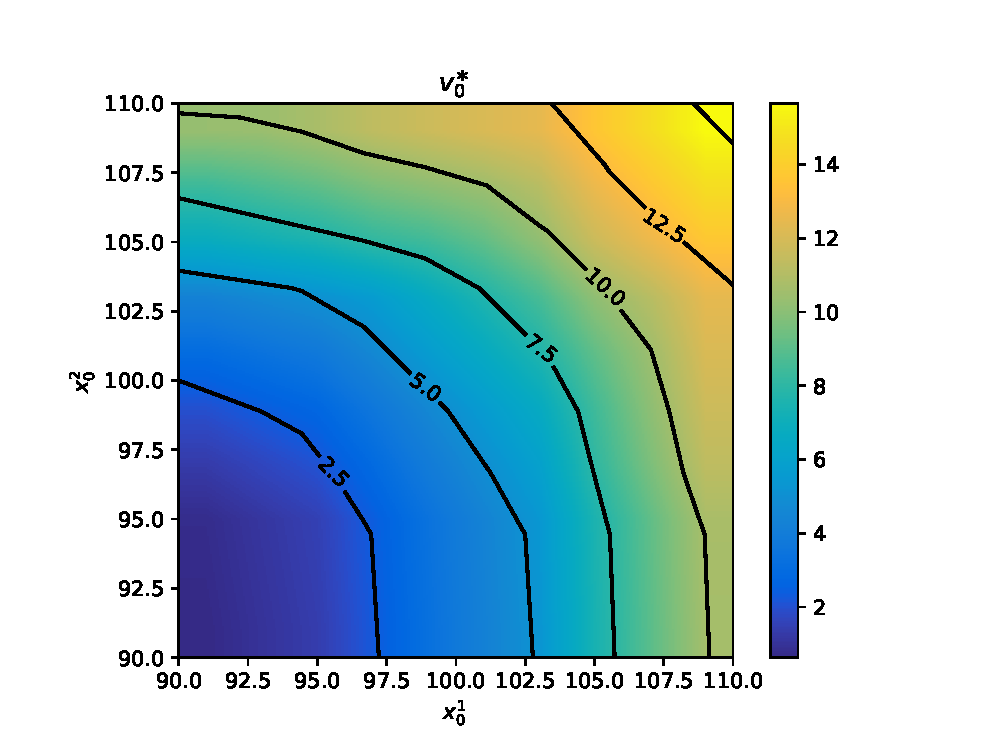
\includegraphics[width=0.5\linewidth]{depends_on_start.eps}
        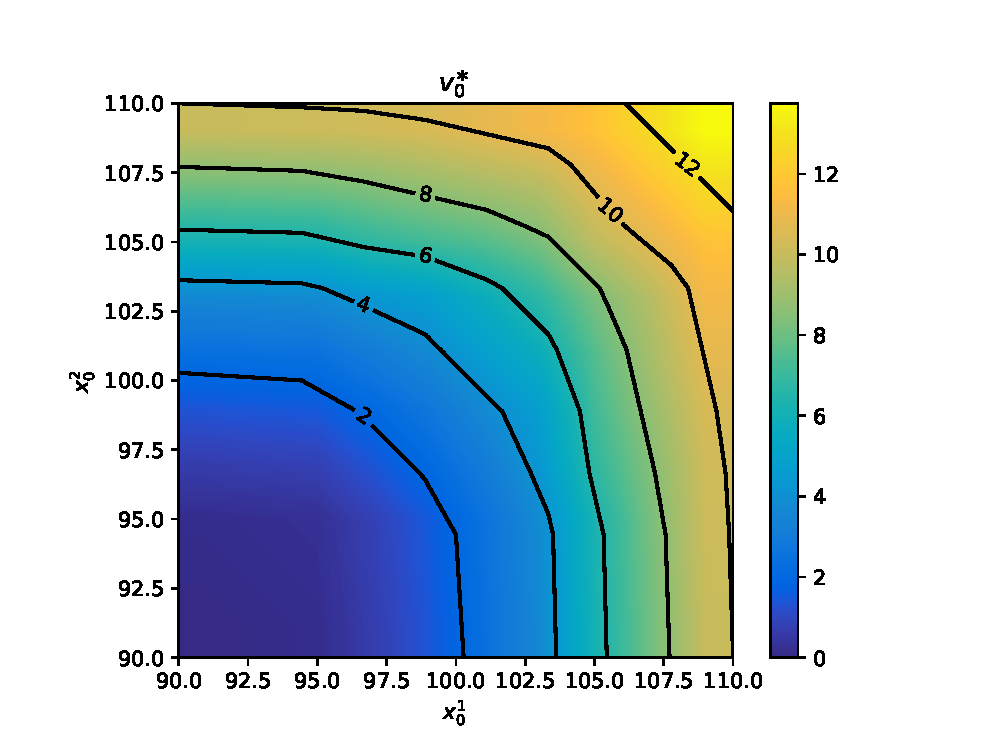
\includegraphics[width=0.5\linewidth]{depends_on_start_equal.eps}
        \caption{Зависимость премии от начальной цены рисковых активов $x_0$. Ограничения слева равны $\Pi=[0,\!97,1,\!03]\times[0,\!99,1,\!01]$, справа~--- $\Pi=[0,\!99,1,\!01]\times[0,\!99,1,\!01]$.}
    \end{figure}

    \begin{figure}[t]
        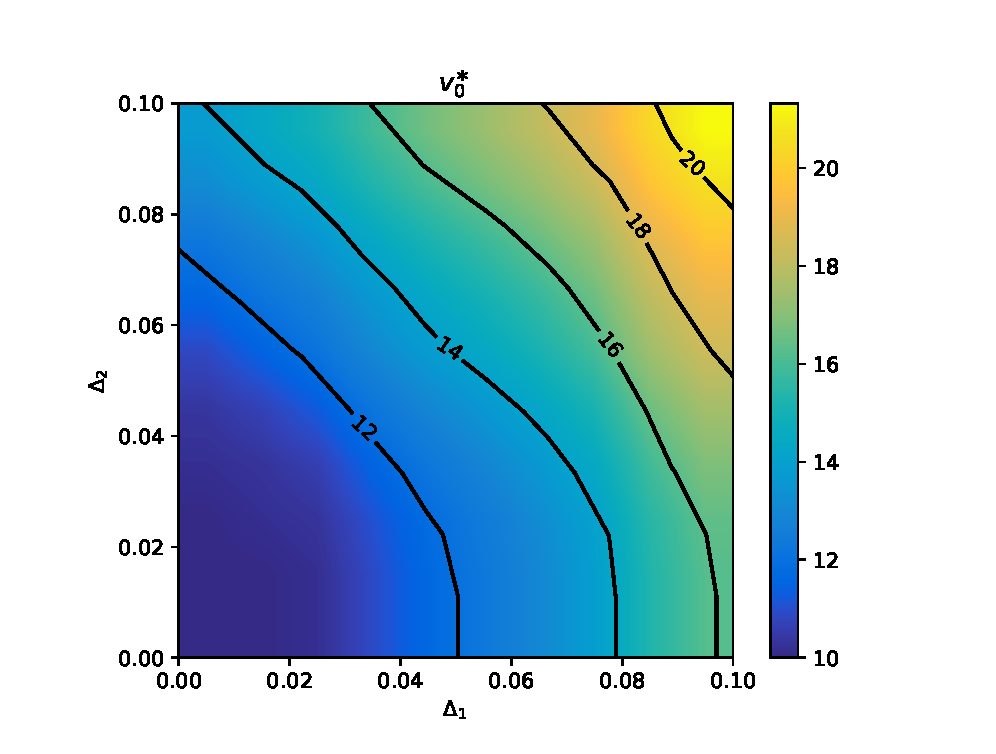
\includegraphics[width=0.5\linewidth]{depends_on_volatility_90_110.eps}
        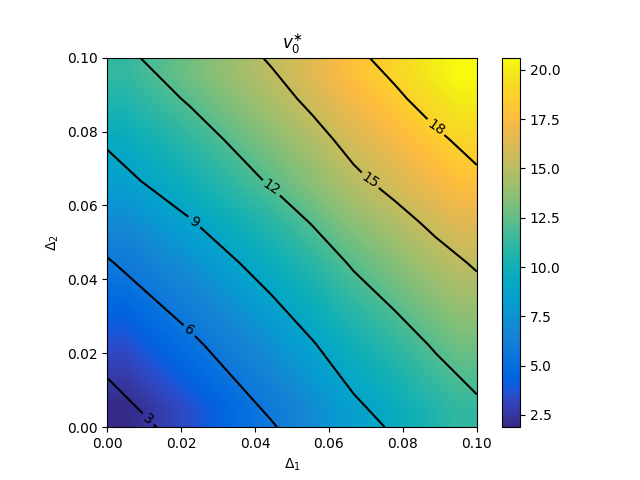
\includegraphics[width=0.5\linewidth]{depends_on_volatility_100_100.png}
        \caption{Зависимость премии от дисперсии рисковых активов, то есть ограничения $\Pi = [1-\Delta_1,1+\Delta_1] \times [1-\Delta_2, 1+\Delta_2]$. Начальная стоимость слева равна $x_0=[90,110]$, справа~--- $x_0=[100,100]$.}
    \end{figure}
\end{document}